\section{Software Ontwerp}
In deze sectie zal het software ontwerp behandeld worden. Dit is het grootste gedeelte van de opdracht. Het software ontwerp bestaat uit twee delen. Er is \gls{PLC} code nodig om alle modules aan te sturen en daarnaast is er frontend code waarmee de gebruiker interfaced. De frontend praat vervolgens weer via \gls{ADS} met de \gls{PLC} zodat deze weet wat er moet gebeuren. Ook worden foutcodes uitgelezen uit de \gls{PLC} zodat de gebruiker weet wat er mis gaat in geval van een error.

\subsection{Software Morfologisch Overzicht}

\begin{xltabular}{\linewidth}{|p{0.3\linewidth}|p{0.2\linewidth}|p{0.2\linewidth}|}
	\caption{Software Morfologisch Overzicht} \\
	\hline
	\textbf{Component} & \textbf{Oplossing 1} & \textbf{Oplossing 2} \\
	\hline
	\endfirsthead
	\hline
	\textbf{Component} & \textbf{Oplossing 1} & \textbf{Oplossing 2} \\
	\hline
	\endhead
	\hline
	\endfoot
	\hline
	\endlastfoot
	\textbf{Frontend Programmeertaal} & \cellcolor{green} C\# WPF XAML & C++/CX XAML \\
	\hline
	\textbf{Backend Programmeertaal} & \cellcolor{green} \gls{TC3} \gls{ST} & \gls{TC3} C++ \\
	\hline
\end{xltabular}

\begin{table}[H]
	\centering
	\caption{Frontend Programmeertaal}
	\label{tab:FrontendProgrammeertaal}
	\begin{tabular}{|p{0.2\linewidth}|p{0.15\linewidth}|p{0.16\linewidth}|p{0.16\linewidth}|}
		\hline
		\multicolumn{4}{|c|}{\textbf{Programmeertaal}} \\
		\hline
		\textbf{Criteria} & \textbf{Wegingsfactor} & \textbf{C\# WPF XAML} & \textbf{C++/CX XAML} \\
		\hline
		Snelheid & 2 & 70 & 90 \\
		Gebruiksvriendelijk & 1 & 90 & 70 \\
		\hline
		\textbf{Totaal} & - & \fpeval{2*70 + 1*90} & \fpeval{2*90 + 1*70} \\ % Automatische berekening
		\hline
	\end{tabular}
\end{table}

Als programmeertaal is C++/CX XAML als beste becijfert die komt omdat de \gls{IPC} op de testkast erg langzaam kan zijn daarom heeft de snelheid veel invloed op de uiteindelijke keuze. Ook is C++ gemakkelijk in geval van het 3D renderen doormiddel van bijvoorbeeld Vulkan dit kan makkelijk zijn om in 3D bijvoorbeeld problemen aan te geven in het model (Voorbeeld figuur \ref{fig:VulkanPOP}). Echter omdat Voortman zelf C\# WPF XAML gebruikt zou het voor onderhoudt en ook wanneer er iets mis gaat slimmer zijn om dit te gebruiken ook al is het minder snel met meer geheugengebruik.

\begin{figure}[H]
	\centering
	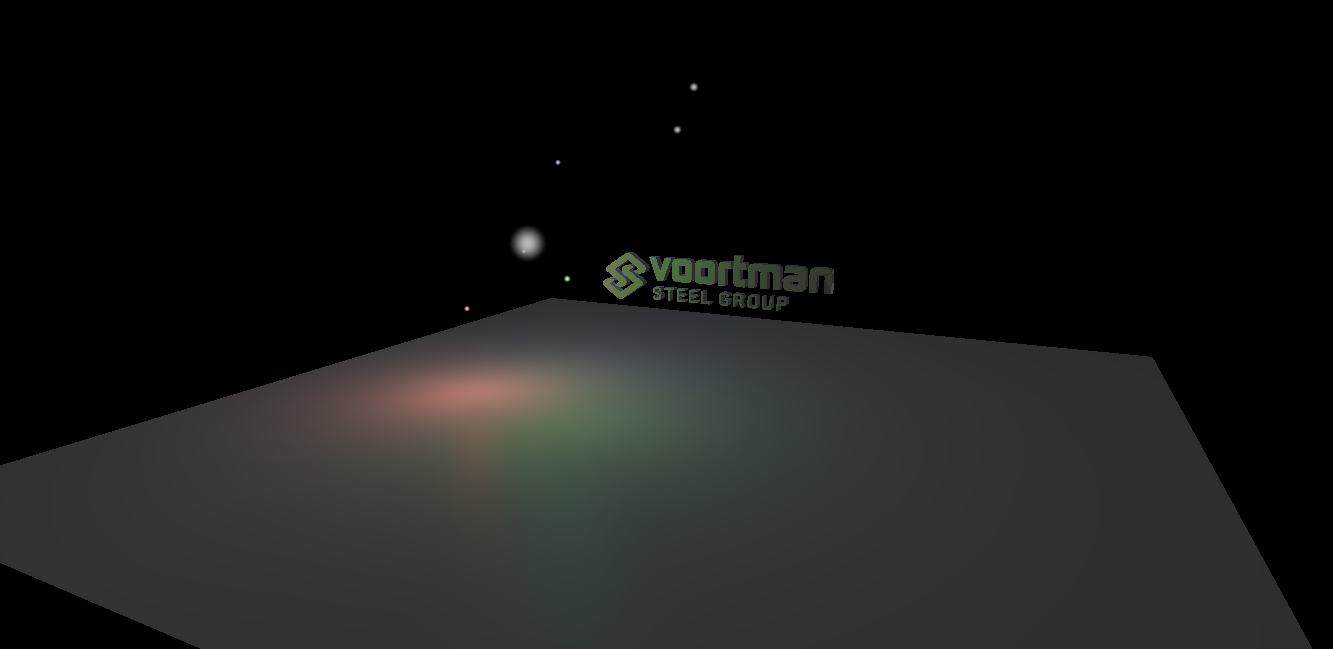
\includegraphics[width=\linewidth]{VulkanPOP}
	\label{fig:VulkanPOP}
	\caption{Proof of Concept 3D render with Vulkan in C++}
\end{figure}

\begin{table}[H]
	\centering
	\caption{Backend Programmeertaal}
	\label{tab:BackendProgrammeertaal}
	\begin{tabular}{|p{0.2\linewidth}|p{0.15\linewidth}|p{0.16\linewidth}|p{0.16\linewidth}|}
		\hline
		\multicolumn{4}{|c|}{\textbf{Programmeertaal}} \\
		\hline
		\textbf{Criteria} & \textbf{Wegingsfactor} & \textbf{\gls{TC3} \gls{ST}} & \textbf{\gls{TC3} C++} \\
		\hline
		Snelheid & 2 & 70 & 90 \\
		Gebruiksvriendelijk & 1 & 90 & 70 \\
		\hline
		\textbf{Totaal} & - & \fpeval{2*70 + 1*90} & \fpeval{2*90 + 1*70} \\ % Automatische berekening
		\hline
	\end{tabular}
\end{table}

Voor de \gls{PLC} code geldt eigenlijk hetzelfde als voor de frontend. Voortman zelf maakt gebruik van zowel C++ als \gls{TwinCAT}. Echter is het alleen aangeraden C++ te gebruiken voor erg intensieve taken zoals collision modellen of beeldverwerking. Aangezien de testkast geen intensieve real-time operaties hoeft te verrichten is het beter om \gls{TwinCAT} te gebruiken vanwege de gebruiksvriendelijkheid en de gemakkelijke integratie met motion control en \gls{IO} \cite{web:PLCC++}.

\subsection{\gls{PLC}}
Deze sectie zal gaan over de \gls{PLC} code van de testkast. Deze code is verantwoordelijk voor het cyclisch updaten van alle componenten en het aansturen hiervan. Daarnaast bevat het systeem ook nog een safety \gls{PLC} die los staat van de andere \gls{PLC} code.

\subsubsection{Safety \gls{PLC}}

\begin{figure}[H]
	\centering
	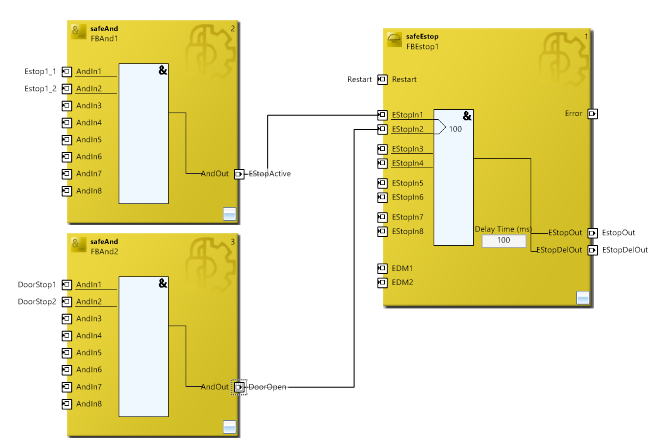
\includegraphics[width=\linewidth]{SafeEStop}
	\caption{Safety \gls{PLC} code}
	\label{fig:SafetyPLC}
\end{figure}

De code van de Safety \gls{PLC} is te zien in figuur \ref{fig:SafetyPLC}. Er wordt hier gebruik gemaakt van vier ingangen van de EL1904. Twee van deze ingangen zijn aangesloten op de emergency buttons en de overige twee zijn van de deurschakelaars. In beide gevallen moet het resulteren in een activatie van de safety kaart in de motordrive daarom zijn de safeAnd functie blokken allebei aangesloten op de safeEStop die twee uitgangen heeft op de EL2904 die aan de safetykaart van de motordrive zit. Om toch onderscheid te kunnen maken in de \gls{PLC} code zijn er ook twee uitgangen aangemaakt die de \gls{PLC} kan uitlezen of de deuren geopent zijn of dat de emergency knop is ingedrukt. De source code van de safety \gls{PLC} maar ook de rest van de code is te vinden in bijlage \ref{sec:SourceCode}.

\newpage

\subsubsection{\gls{PLC} code}

Voortman heeft voor de algemene structuur en voor veel gebruikte objecten in de \gls{PLC} een \gls{BaseLib} gemaakt. Deze \gls{BaseLib} zal ook gebruikt worden in de \gls{PLC} code van de testkast zodat er een bekende en soortgelijke structuur ontstaat als in de machines van Voortman. 

\subsection{Frontend code}

De frontend code is 